\chapter[Introduction]{Introduction}
\label{ch:intro}
\containsfigures{Introduction}
\containslistings{Introduction}
\containstables{Introduction}

\chapterepigraph{Advances in technology won't be as significant as they have been in the past, most games won't be materially improved by simulating every drop of water in the pond you are wading through. More resources can be profitably spent to make the creation process easier.}{John Carmack}

\newthought{Functional programming} (FP) has a long history, with its roots in the $\lambda$-calculus of Alonzo Church.\citefix[-1.5em]{church1932} One of the first functional programming languages was Lisp, invented by John McCarthy in 1958, which is still used today, over 50 years later.\citepage{reilly2003}{pages 156--157} Various languages have refined and extended the functional paradigm over the years --- probably the most notable as of now being Haskell, Scala, OCaml, F\#, and Erlang.

\begin{marginfigure}
	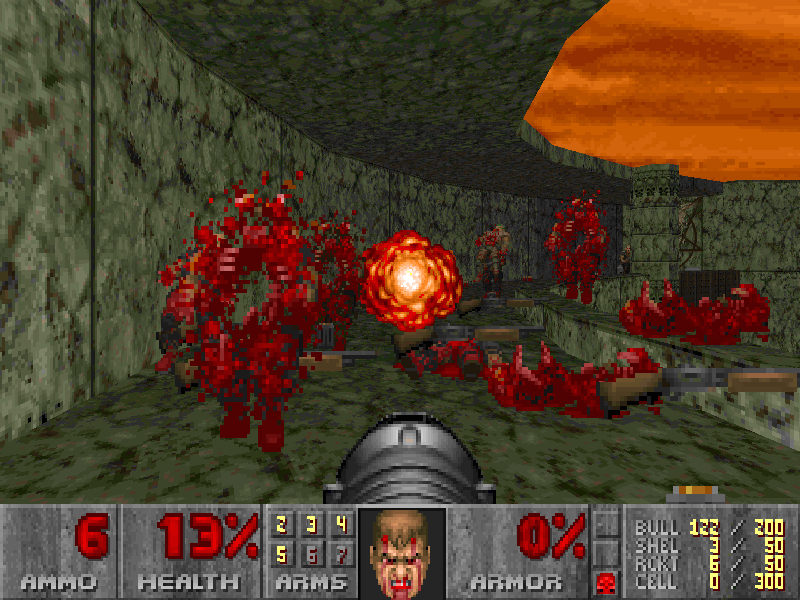
\includegraphics[width=6cm]{res/doom/doom.png}
	\caption[A screen from \emph{Ultimate Doom}.]{A screen from \emph{Ultimate Doom} (1995). Extended caption etc.}
	\label{fig:doom}
\end{marginfigure}

\lipsum[1]

\lipsum[4]

\begin{table*}[t]
	\footnotesize
	\renewcommand{\arraystretch}{1.5}
	\begin{tabular}{p{9em} p{5em} p{3em} p{3em} p{9em} p{9em} p{9em}}
		\toprule
		\emph{Stakeholder} & \emph{Relationship} & \emph{Power} & \emph{Interest} & \emph{Requirements} & \emph{Measurements} & \emph{Communication Strategy} \\
		\midrule
		
		Project Team & Internal & High & High & 
		Good working environment, creative input. & 
		Meeting project spec, good grades! & 
		Various, detailed elsewhere. \\
		
		Supervisor --- Sara Kalvala & Internal & High & High & 
		Good communication. & 
		Adherence to spec, good PM, high quality write-up. & 
		Weekly meetings. \\
		
		Client --- Matt Leeke & Core \mbox{External} & High & High & 
		Good communication, creative input, hard work & 
		Strength of software, strength of report & 
		Weekly meetings. \\
		
		Second Assessor & Core \mbox{External} & High & Low & 
		None & 
		Marking scheme & 
		Deliverables only. \\
		
		Projects Organiser --- Steve Matthews & External & High & Low & 
		Cooperation when required. & 
		Deliverables on time. & 
		Email or meeting if required. \\
		
		Playtesters & External & Low & High & 
		Able to report issues / feature requests. & 
		Strength of game, input considered. & 
		Email. \\
		
		Other future users & Rest of World & Low & High & 
		Game works and is reliable. & 
		Strength of game, re-playability. & 
		Website, forums, blog. \\
		
		The Haskell and FP Communities & Rest of World & Low & High & 
		None & 
		Interest in  / strength of results and tools released. & 
		Online as above, and via the final report. \\
		\bottomrule
	\end{tabular}
	\vspace{1.5em}
	\caption[][1em]{Stakeholders for the project.}
	\label{tab:stakeholders}
\end{table*}

\section{Typesetting Haskell}

Lambda\TeX\ is written for \TeX\ rather than \LaTeX, and so works a little differently from how you might expect. It is designed to typeset Literate Haskell documents and so uses an angle brace to denote a haskell line

> this is a Haskell line
> data List a = Cons a |Empty

To control the spacing and other parameters around these lines I have made a \emph{haskell} environment to be used like this.

\hasklisting{list:reduce}{The \emph{reduce} function}{The \scalenote{"reduce"} function. Extended caption.}

\vspace{-1em}
\begin{listing}{list:reduce}{The \emph{reduce} function}{The \scalenote{"reduce"} function. Extended caption.}{}
\end{listing}\vspace{-1em}

\functions(reduce)
\begin{haskell}
>reduce :: (state -> alphabet -> state) -> state -> [alphabet] -> state
>reduce delta q0 []     = q0

\marginnote{\anote This definition uses pattern matching on the string being passed to split it into head and tail parts; ie the pattern \scalenote{"(x:xs)"} results in \scalenote{"x"} being the character at the head of the list and \scalenote{"xs"} the remaining list. }\vspace{-1.7em}
>reduce delta q0 (x:xs) = reduce delta (delta q0 x) xs

\end{haskell}
\noindent
The function command is to tell Lambda\TeX\ the names of functions as it couldn't otherwise work them out without a full Haskell parser. The lack of extra newlines around the end of the haskell environment and the \textbackslash noindent is required. The example above also shows how to embed a code annotation as a margin note. 

Inline haskell code is put between double tick marks ie "reduce delta q0". (Use a single tick twice for a normal closing quotation mark.) 

Lastly, Lambda\TeX\ will not react to normal text scaling commands as these are part of \LaTeX, so a scaling command must be added when setting Haskell within sidenotes or anywhere with a different text size.


